\chapter{Game Analysis}

In Chapter \ref{GameDescription}, we briefly explored the rules and gameplay mechanics of Quoridor.
As we progress, this chapter aims to deepen our understanding by analyzing Quoridor from a
theoretical and computational perspective.

In this chapter will classify Quoridor within the realm of strategic games, examine its game tree,
state-space and tree complexity, and explore the implications of these factors on gameplay and
artificial intelligence application.

\section{Classification of Quoridor}

Quoridor can be characterized as a discrete, deterministic, zero-sum, sequential, game with perfect
information (\cite{Glendenning2002MasteringQ}) , and therefore, a combinatorial game (\cite{GameTheoryBook})

\subsection{Discrete}
In every turn, each player has a finite number of moves and wall placements. These are limited by the
game state (already placed walls and moved pawns) and the rules of the game. The game-tree of Quoridor
has finite number of nodes (e.g \ref{fig:GameTree})

\subsection{Deterministic}
Quoridor has no random elements or chance involved in the gameplay. Every outcome and situation
is a direct result of the players' decisions and strategies. There's no dice rolling,
card drawing, or any other mechanism that introduces randomness.

\subsection{Zero-sum}
In Quoridor, when a player makes a move that brings them closer to winning (like advancing their pawn
or placing a wall effectively), it inherently puts the opponent at a disadvantage. Therefore, any
positive progress for a player translates into a negative impact for their opponent. This reciprocal
relationship of gain and loss between the players is what characterizes Quoridor as a \textbf{zero-sum} game.

\subsection{Perfect Information}
Every aspect of its gameplay are completely visible and known to all players at all times. This means
that the positions of the pawns and the placements of the walls on the board are always in full view,
allowing players to make strategic decisions based on the entire state of the game.

\newpage

\section{Game-Tree}

A game tree for an \textbf{abstract strategy game} is a comprehensive graph representing every possible game states and sequence of moves. The nodes of a game tree represent game states, and the
edges represent action/move.

Game trees are integral to the framework of \textbf{adversarial search problems}, where they are employed to systematically explore and evaluate the possible outcomes of different strategies, and forecast future states of the game based on current and potential moves.
\newline
\newline
The following depicts a (partial) game tree for the Quoridor game with a board of size 3x3:

\begin{figure}[h]
    \centering
    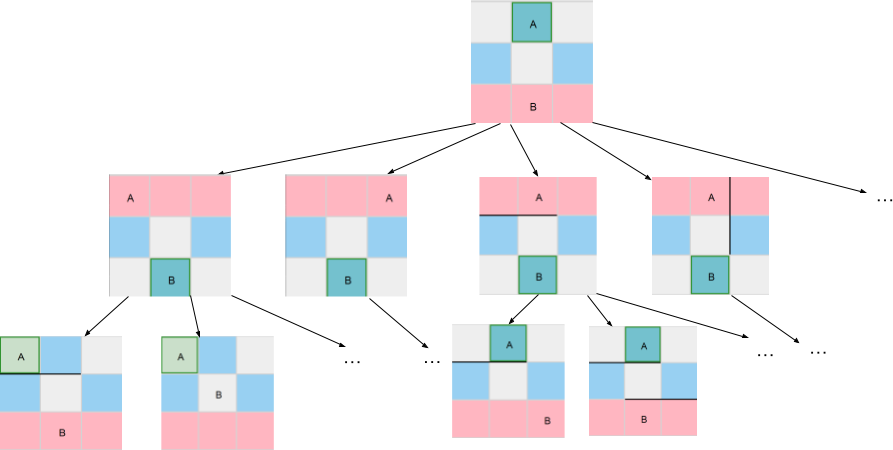
\includegraphics[scale=0.45]{../img/GameBoard/game_tree.png}
    \caption{A partial game tree for a 3x3 game board.}
    \label{fig:GameTree}
\end{figure}

\subsection{Branching Factor}
\label{BranchingFactor}

The branching factor of a \textbf{Game-tree} is the number of child nodes of each node, or in other words, the number of possible moves a player at their turn can make, given the game state.

In figure \ref{fig:GameTree}, player A makes the first move. A has \textbf{3} places to move their pawn to and \textbf{8} places to put one of their walls at. So, the root has a \textbf{branching factor} of \textbf{11}.
\par
The branching factor is greatly influenced by the state of the board in Quoridor, i.e the player locations and walls placed.
\newline
\newline
As an example, the figure below represents a game states with the maximum and minimum branching factors:

\begin{figure}[h]
    \begin{subfigure}{0.4\textwidth}
      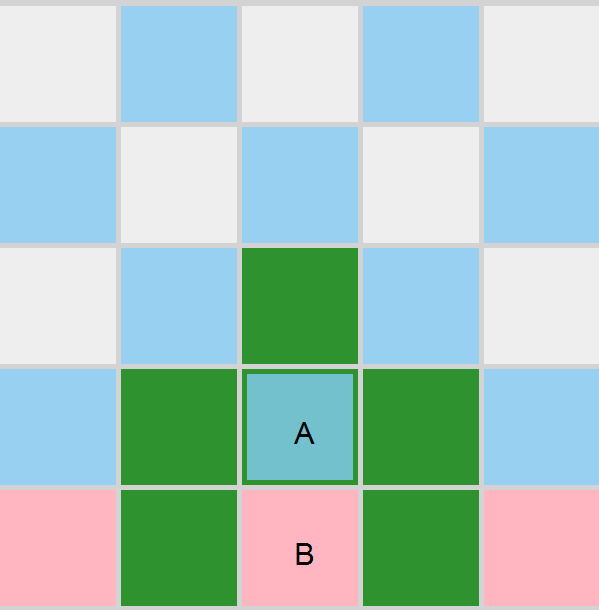
\includegraphics[width=\textwidth]{../img/GameBoard/maximum_branching_factor.png}
      \caption{Maximum : 37}
      \label{fig:MaxBranchingFactor}
    \end{subfigure}
    \hfill
    \begin{subfigure}{0.4\textwidth}
      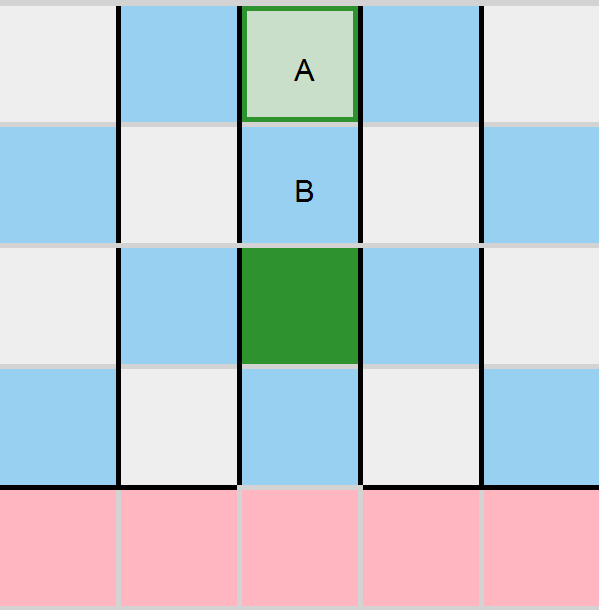
\includegraphics[width=\textwidth]{../img/GameBoard/minimum_branching_factor.png}
      \caption{Minimum : 1}
    \end{subfigure}
    \caption{Branching factor differences}
    \label{fig:MinBranchingFactor}
\end{figure}

As depicted by Figure \ref{fig:MaxBranchingFactor}, player A has 5 possible places to move their pawn to. No walls have been placed so far, so player A can also place one of their walls in any place.
\par
For a board of size NxN with no wall(s) placed, $(N-1)$ walls can be placed in each row (since each wall occupies \textbf{2} cell lengths), and there are $(N-1)$ rows for correct horizontal wall placements. Hence, there are $(N-1)^2$ slots for horizontal wall placements, and since the board is NxN, the total  slots for both horizontal and vertical wall placements is given by the equation:
\begin{equation}
\label{eq:WallPlacements}
    2*(N-1)^2
\end{equation}

\par
Coming back to figure \ref{fig:MaxBranchingFactor}, since the board has no walls placed, we now see that A has $5 + 2*(5-1)^2 = 37$ possible moves they can perform, ergo, the branching factor of the game state represented by Figure \ref{fig:MaxBranchingFactor} is \textbf{37}, which is also the maximum branching factor for board sized 5x5.
\newline
\newline
However, in Figure \ref{fig:MinBranchingFactor}, A has no available slot for wall-placement, and the already present walls block A from moving anywhere except for cell \textbf{c3}. Hence, the branching factor for the game state represented by Figure \ref{fig:MinBranchingFactor} is 1.

\subsubsection{Average Branching Factor}

In sub-section \ref{BranchingFactor}. we saw that the branching factor is not uniform due factors like wall-placements and positioning of the player greatly influencing it.
\par
We, therefore, would like to estimate an average branching factor for boards of different lengths to see if varying board dimension has any affect in the average branching factor.
\par
We already know from equation \ref{eq:WallPlacements} that the maximum branching factor of the game tree is exponential in order of $N$ and from Figure \ref{fig:MinBranchingFactor}, we can deduce that the minimum branching factor is 1 (since we can replicate a similar game state for any game state).

To find an estimate of the average branching factor, we use the Algorithm \ref{alg:AverageBranchingFactor}

\begin{algorithm}[H]
\caption{Average branching factor}
\label{alg:AverageBranchingFactor}
\DontPrintSemicolon
\SetKwInOut{Input}{input}\SetKwInOut{Output}{output}
\SetKwFunction{FMain}{AvgBranchingFactor}
\SetKwProg{Fn}{Function}{:}{}
\Fn{\FMain{agent1, agent2, simulations}}{
    \Input{Two agents and number of simulations}
    \Output{Average of averages branching factor}
    SumOfAverages $\gets$ 0\;
    \For{i $\gets$ 1 \KwTo simulations}{
        State $\gets$ Initialize()\;
        GamePossibleMoves $\gets$ 0\;
        GameMovesMade $\gets$ 0\;
        Agents $\gets$ [agent1, agent2]\;
        AgentIndex $\gets$ 0\;
        \While{State is not Terminal}{
            Agent $\gets$ Agents[AgentIndex]\;
            AgentIndex $\gets$ (AgentIndex + 1) \% 2\;
            GamePossibleMoves $\gets$ GamePossibleMoves + Length(State.PossibleMoves())\;
            Move $\gets$ Agent.GetMove(State)\;
            State $\gets$ State.Apply(Move)\;
            GameMovesMade $\gets$ GameMovesMade + 1\;
        }
        GameAverage $\gets$ GamePossibleMoves / GameMovesMade\;
        SumOfAverages $\gets$ SumOfAverages + GameAverage\;
    }
    \KwRet SumOfAverages / simulations\;
}
\end{algorithm}

\newline

We then simulate \textbf{1000} games between \textbf{Minimax AB} and \textbf{Semi-random} agents, each for boards of dimensions 3, 5, 7 and 9, and the results of the average branching factor can be seen in figure \ref{fig:BranchingFactor}

\begin{figure}[h]
    \centering
    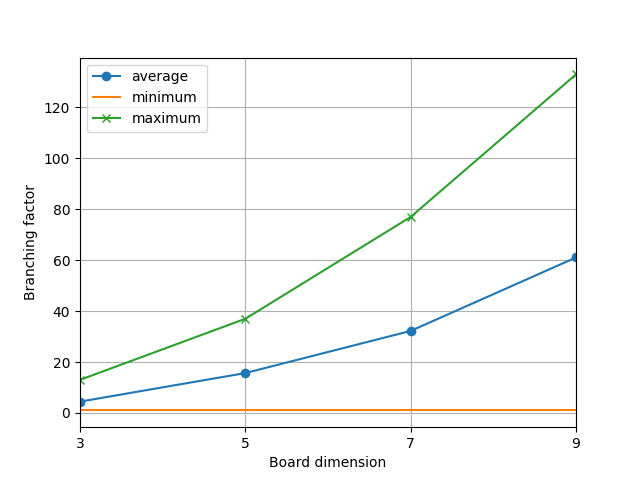
\includegraphics[scale=0.6]{../img/branching_factor.png}
    \caption{Branching factor for boards of different sizes}
    \label{fig:BranchingFactor}
\end{figure}

From figure \ref{fig:BranchingFactor}, like with the maximum branching factor, we can see a similar exponential trend of the average branching factors in order of N. Furthermore, based on only the four dimensions and their averages and maximum branching factors, the average branching factor seems to be almost half the maximum branching factor

The average branching factor for board of dimension 9x9 was about \textbf{62}, which is very close to the value proposed by \cite{Glendenning2002MasteringQ}